\chapter{Appendix}\label{appendix}
Here we will lay out the details of the architecture and hyperparameter settings that were used in each agent mentioned in section \ref{research-method}. We start with the agents for the Starcraft II environment, then secondly the OpenAI Atari Pong environment.

\section{Starcraft II: RL agent architectures}\label{appendix-agents}
In this section we will give the specific architecture and hyperparameter settings used for RL agents in the Starcraft II environment. We will start by showing the baseline agent, which uses an architecture and hyperparameters that are shared by all agents. For all other agents, each extending this baseline agent, we will only give the additional architecture and parameters. For an overview of how each agent works, we refer to sections \ref{research-exp} and \ref{research-env-pysc2}.


\subsection{Baseline agent}\label{appendix-baseline}
\textbf{Neural network architecture}\newline
\noindent The DDQN policy and target network for the baseline agent consists of a CNN with three convolutional layers. The first layer is a transposed convolutional layer \cite{transpose} and the other two are regular convolutional layers. The transposed convolutional layer has the possibility to upscale the dimensionality, which is needed in agents using dimensionality reduction. These agents have their observation reduced from $32 \times 32$ to $16 \times 16$. This $16 \times 16$ observation is the input for their policy and target network. The output of these networks however need to be $32 \times 32$, capturing the action space. Although this upscaling is not needed for the baseline agent since it uses the full $32 \times 32$ observation as input, we still use it as the first layer in order to keep all agents' architectures as similar as possible.

Each layer uses a stride of $1$, input padding of $1$ and no output padding, keeping the dimensionality of the input the same. Furthermore, they also each have a kernel size of $3$. The first layer has $32$ output channels. The second layer has $32$ input channels (following the output channels of its previous layer) and $32$ output channels. The third and last layer has $32$ input channels (again following the output channels of its previous layer) and $1$ output channel. Both after the second and the first layer, we use the activation function known as \emph{ReLU} \cite{relu} whose output for each neuron is defined as the maximum of $0$ and the input neuron.

When training the policy network, the optimization algorithm \emph{Adam} is used, which is an extension on \emph{stochastic gradient descent} \cite{adam}. For loss calculation we refer to section \ref{pl-dqn}, more specifically algorithm \ref{alg:ddqn}.

\noindent\textbf{Hyperparameters}\newline
\noindent The following hyperparameters are used in the baseline agent:
\begin{itemize}
\item Steps in between training the policy network: $4$.
\item Steps between updating the target network: $250$.
\item Optimizer learning rate: $0.0001$.
\item Discount factor: $0.99$.
\item Batch size for training the policy network: $256$.
\item Number of stored batches before training: $20$.
\end{itemize}

Lastly, an $\epsilon$-greedy strategy is used for balancing exploration and exploitation. This means that a random number in $[0,1]$ is chosen; whenever this is equal to or lower than the current epsilon value, a random action is chosen, and a greedy action otherwise. Epsilon decays from $1.0$ to $0.1$ in $100.000$ steps spaced on a logarithmic scale. Each step taken by the agent corresponds to one epsilon decay step. The resulting decay of the epsilon value can be seen in figure \ref{fig:epsilon}.

\begin{figure}[h]
    \centering
    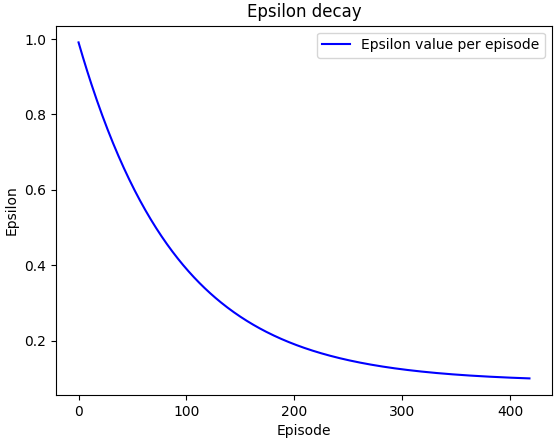
\includegraphics[width=0.75\textwidth]{Epsilon_decay}
    \caption{The decay of the epsilon value per episode.}
    \label{fig:epsilon}
\end{figure}

\subsection{PCA agent}
The neural network architecture and hyperparameter settings of the PCA agent are almost exactly the same as the baseline agent (see appendix \ref{appendix-baseline}). The only difference is that in the policy and target network, the first layer (the transposed convolutional layer) now has a stride of $2$ and output padding of $1$. This is to upscale dimensionality from the $16 \time 16$ observation (gotten after dimensionality reduction using PCA) to $32 \times 32$ representing the action space.


\subsection{Pre-trained and online trained autoencoder agent} %TODO "online"
Like with the PCA agent, the difference with the baseline agent with regards to the DDQN architecture is merely the first layer of the policy and target network of the agent: it now has a stride of $2$ and output padding of $1$ to upscale the dimensionality from its $16 \times 16$ input to $32 \times 32$ output. In both autoencoder agents, the autoencoder has the same architecture and hyperparameters. \newline

\noindent \textbf{Autoencoder neural network architecture and hyperparameters}
\noindent The encoder of the autoencoder consists of two convolutional layers. The first layer has a stride of $2$ to introduce dimensionality reduction from $32 \times 32$ to $16 \times 16$. The second layer has a stride of $1$ to keep this $16 \times 16$ dimensionality. Both layers have a kernel size of $3$ and an input padding of $1$. The first layer has $1$ input channel (since the observation input only has one channel) and $32$ output channels. Hence, the second layer has $32$ input channels and $1$ output channel. After both layers, there is a \emph{GELU} activation function, which is a nonlinear variant of ReLU \cite{gelu}.

The decoder consists of three layers. Because the decoder has to reconstruct the original input from the output of the encoder, the first is a transposed convolutional layer to upscale its $16 \times 16$ input back to $32 \times 32$. This is done using a stride of $2$ and output padding of $1$. It has $1$ input channel (corresponding to the $1$ output channel of the last encoder layer) and $32$ output channels. The other two layers are regular convolutional layers, with stride $1$ and no output padding. For the second layer, there are $32$ input and output channels, and for the third and last layer there are $32$ input channels and $1$ output channel (corresponding to the $1$ input channel of the first layer of the policy and target network). Each layer has a kernel size of $3$ and input padding of $1$. After the first and second layer there is a GELU activation function.

For training the autoencoder, the loss is calculated by the mean-scared-error between the original input and the reconstructed input. Furthermore, the Adam optimization algorithm is used, with a learning rate of $0.0001$. 


\subsection{DeepMDP agent}
Compared to the baseline agent, the policy and target network of the DeepMDP agent have a prepended encoder. Furthermore it has an additional neural network for the transition loss (i.e. the auxiliary objective). Apart from these changes (including a different loss calculation) the only difference with the baseline agent is again the first layer of the target and policy network that now has a stride of $2$ and output padding of $1$ to upscale the dimensionality from $16 \times 16$ to $32 \times 32$. \newline

\noindent \textbf{DeepMDP encoder and transition loss architectures and hyperparameters} \newline
\noindent The encoder has the same architecture as the encoder in the autoencoder agents. It has two convolutional layers, with the first layer having a stride of $2$ for dimensionality reduction. The first layer has $1$ input channel and $32$ output channels and vice versa for the second layer. Both have a kernel size of $3$ and input padding of $1$. After both layers the activation function GELU is used.

The transition loss neural network has only $1$ layer, a convolutional layers. Most importantly, it has $1024$ output channels, corresponding to the $32 \times 32$ action space. It has a stride of $1$ and kernel size $2$.

Besides the usual DDQN loss calculation as with the baseline agent, the DeepMDP has an additional loss added to this; this total loss is used to train all neural networks of the DeepMDP. The transition loss is calculated by comparing the prediction of the next observation after dimensionality reduction given by the transition loss network, with the actual next observation after dimensionality reduction (i.e. the output of the encoder). The loss is calculated using the L1 loss function \cite{l1}. Added to this loss, is the gradient penalty which is discounted by a hyperparameter set to $0.01$. The gradient penalty is a combination of the gradient penalty of the encoder, the policy network and the transition loss network. For each of these three networks, the penalty is calculated using the Wasserstein Generative Adversarial Network penalty \cite{wgan}.

\section{OpenAI Pong: RL agent architectures}\label{appendix-agents-pong}
%TODO pong: explain policy network image reduction?
In this section we will give the specific architecture and hyperparameter settings used for RL agents in the OpenAI Atari Pong environment. We will start by showing the baseline agent, which uses an architecture and hyperparameters that are shared by all agents. For all other agents, each extending this baseline agent, we will only give the additional architecture and parameters. For an overview of how each agent works, we refer to sections \ref{research-exp} and \ref{research-env-pong}.


\subsection{Baseline agent}\label{appendix-baseline-pong}
\textbf{Neural network architecture}\newline
\noindent The DDQN policy and target network for the baseline agent consists of three convolutional layers and two linear layers. Its input is $n \times 4 \times 84 \times 84$, for batches of size $n$. The $4$ channels represent the four consecutive frames that are used for a single observation. Each convolutional layers has no padding. The strides for each layer is $6$, $4$ and $3$ respectively, and the kernel/filter sizes are $3$, $2$ and $1$ respectively. The first layer has 4 channels, one for each input frame. It has $32$ output channels, thus the second layer has $32$ input channels. The second layer has $64$ output channels, thus the third layer has $64$ input channels. This last convolutional layer also has $64$ output channels. For input with batch size $n$, the downsampling through the convolutional layers is from $n \times 4 \times 84 \times 84$, to $n \times 32 \times 27 \times 27$, to $n \times 64 \times 12 \times 12$ to $n \times 64 \times 10 \time 10$. 

The output after the last convolutional layer is flattened to $n \times (64 \cdot 10 \cdot 10) = n \times 6400$, which will be the input for the first linear layer. Thus, the first linear layer has $6400$ input features. It has $512$ output features. The second linear layer has $512$ input features and $6$ output features, covering the action-space. Furthermore, after each convolutional layer, there is batch normalisation layer to normalise the layer outputs \cite{batchnorm}, and a ReLU activation function \cite{relu}. After the first linear layer there is only a ReLU activation function. No activation function or batch normalisation is used after the final layer.

When training the policy network, the optimization algorithm \emph{Adam} is used, which is an extension on \emph{stochastic gradient descent} \cite{adam}. For loss calculation we refer to section \ref{pl-dqn}, more specifically algorithm \ref{alg:ddqn}.

\noindent\textbf{Hyperparameters}\newline
\noindent The following hyperparameters are used in the baseline agent:
\begin{itemize}
\item Steps in between training the policy network: $1$.
\item Steps between updating the target network: $1000$.
\item Optimizer learning rate: $5e-5$.
\item Discount factor: $0.97$.
\item Batch size for training the policy network: $32$.
\item Number of stored batches before training: $313$.
\end{itemize}

Lastly, an $\epsilon$-greedy strategy is used for balancing exploration and exploitation. This means that a random number in $[0,1]$ is chosen; whenever this is equal to or lower than the current epsilon value, a random action is chosen, and a greedy action otherwise. Epsilon decays from $1.0$ to $0.02$ in $400.000$ steps spaced on a logarithmic scale. Each step taken by the agent corresponds to one epsilon decay step. One episode takes roughly between $800$ and $3000$ steps (depending on the length of the episode). The resulting decay of the epsilon value can be seen in figure \ref{fig:epsilon}.

\begin{figure}[h]
    \centering
    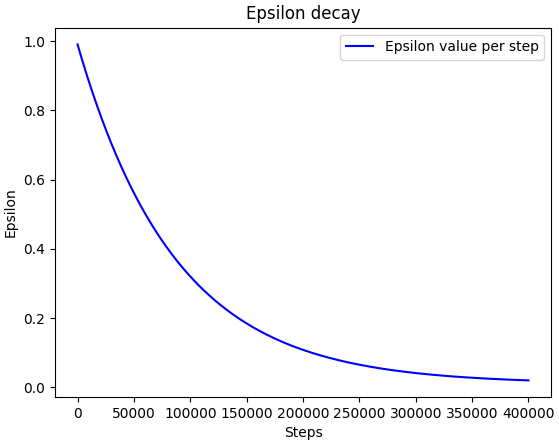
\includegraphics[width=0.75\textwidth]{Pong/Epsilon_decay_pong}
    \caption{The decay of the epsilon value per episode in Pong.}
    \label{fig:epsilon}
\end{figure}

\subsection{PCA agent}
The neural network architecture and hyperparameter settings of the PCA agent are exactly the same as the baseline agent (see appendix \ref{appendix-baseline-pong}). In the PCA agent though, the input for the policy network is now $n \times 4 \times 42 \times 42$, having reduced the dimensionality of each frame from $84 \times 84$ to $42 \times 42$. In the policy network, because of the stride and filter size settings in the convolutional layer, this input is downsampled from $n \times 4 \times 42 \times 42$, to $n \times 32 \times 13 \times 13$ after the first layer, to $n \times 64 \times 5 \times 5$ after the second layer, to $n \times 64 \times 3 \times 3$ after the third convolutional layer. Thus, the first linear layer has $64 \cdot 3 \cdot 3 = 576$ input features.


\subsection{Pre-trained and online trained autoencoder agent} %TODO "online"
Like with the PCA agent, the policy network and hyperparameter settings are the same as the baseline agent \ref{appendix-baseline-pong}. Again, the input for the policy network is now $n \times 4 \times 42 \times 42$, which is downsampled through the convolutional layers to $n \times 64 \times 3 \times 3$. \newline

\noindent \textbf{Autoencoder neural network architecture and hyperparameters}
\noindent The \emph{encoder} of the autoencoder consists of three convolutional layers. The first layer has a stride of $2$ to introduce dimensionality reduction from $84 \times 84$ to $42 \times 42$. The second and third layer have a stride of $1$ to keep this $42 \times 42$ dimensionality. All three layers have a kernel size of $3$ and an input padding of $1$. The first layer has $1$ input channel (since the frame input only has one colour channel) and $32$ output channels. Hence, the second layer has $32$ input channels, and it has $32$ output channel. The third convolutional layer has $32$ input channels and $1$ output channel. After each convolutional layer, there is a \emph{GELU} activation function, which is a nonlinear variant of ReLU \cite{gelu}.

The \emph{decoder} consists of two layers. Because the decoder has to reconstruct the original input from the output of the encoder, the first is a transposed convolutional layer to upscale its $42 \times 42$ input back to $84 \times 84$. This is done using a stride of $2$ and output padding of $1$. It has $1$ input channel (corresponding to the $1$ output channel of the last encoder layer) and $32$ output channels. The other layer is a regular convolutional layers, with stride $1$ and no output padding. For this second convolutional layer, there are $32$ input channels and $1$ output channel (corresponding to the $1$ colour channel of a frame). Each layer has a kernel size of $3$ and input padding of $1$. After the first layer there is a GELU activation function.

For training the autoencoder, the loss is calculated by the mean-scared-error between the original input and the reconstructed input. Furthermore, the Adam optimization algorithm is used, with a learning rate of $0.0001$. 
